% !TeX root = main.tex

\documentclass[a4paper, 11pt]{article}

\usepackage[utf8]{inputenc}
\usepackage[T1]{fontenc}
\usepackage[english]{babel}
\usepackage{setspace}
\usepackage{geometry}
\usepackage{graphicx}
\usepackage{amsmath}
\usepackage{hyperref}
\usepackage{booktabs} 
\usepackage[numbers]{natbib}
\usepackage{listings}
\usepackage{xcolor}
\usepackage{float}

% Only for example text
\usepackage{lipsum}



\title{Example Document}
\author{Author Name}

\graphicspath{{./figures/}}
\geometry{top=3.0cm, bottom=2.5cm, left=3.0cm, right=2.0cm}
\setlength{\headheight}{15pt}
\setlength{\parindent}{0pt}



\begin{document}

\maketitle

\begin{figure}[H]
    \centering
    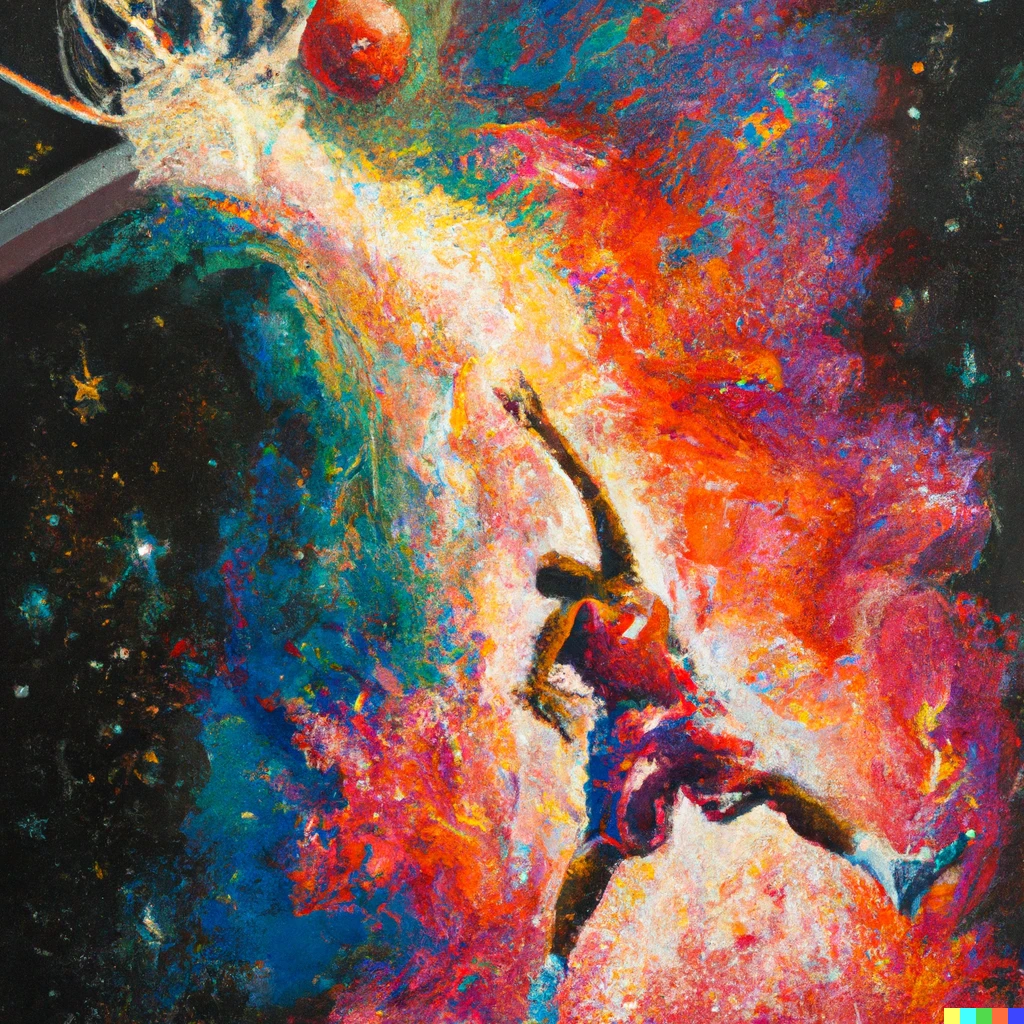
\includegraphics[width=0.5\linewidth]{painting.png}
    \caption{Example Image}
    \label{fig:example-image}
\end{figure}

\tableofcontents
\listoffigures
\newpage


\section{Example Section}

\lipsum[2-5] 
\cite{lorem-ipsum}
\newpage


\bibliographystyle{IEEEtranN}
\bibliography{references}

\end{document}
